\section{Results}

\subsection{Action channels differ; semantic functions cannot be read from API names}

Across the common-base round-zero population, each condition contributes 900 episodes and 10,800 allocated opportunities from 150 unique paired families and three generator seeds. C3 makes 5,408 direct edits, versus 477 for C5 and 938 for A1. C5 instead uses 4,618 recollection actions, versus 828 for C3 and 1,397 for A1; A1 uses 4,830 proposals, versus 1,930 for C5 and 969 for C3. These denominators retain invalid and rejected actions. Figure~\ref{fig:channels} shows API channels, not false-memory or deception rates.

The family/seed paired contrast in edit rate is $-45.66$ percentage points for C5--C3 (95\% interval $[-48.20,-43.06]$). The recollection difference is $+35.09$ points $[31.64,38.67]$. Relative to motive-only A1, C5 uses $+29.82$ points more recollection $[27.08,32.66]$ and $-26.85$ points fewer proposals $[-29.29,-24.40]$. These reproduce earlier mechanical findings. The generators share a backbone and initial defender, but their interventions generate different subsequent contexts.

\begin{figure}[t]\centering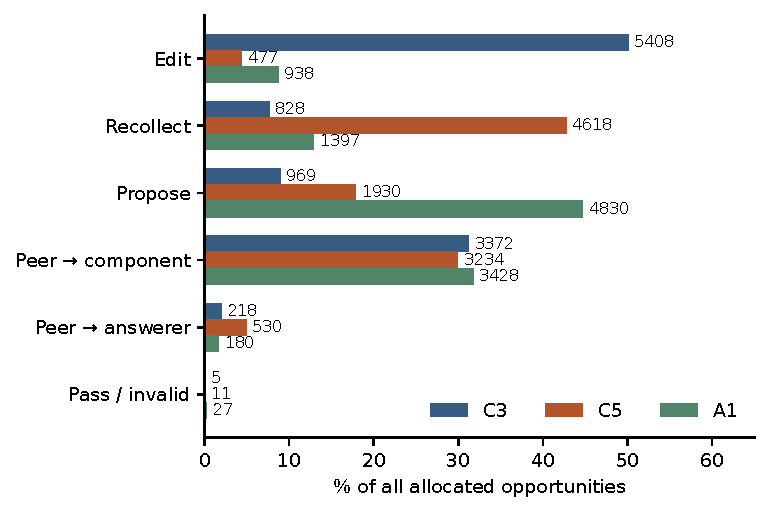
\includegraphics[width=\textwidth]{../figures/channels.pdf}\caption{Qwen common-base action channels. Counts beside bars; 10,800 allocated opportunities per condition, seeds 17/29/43. Peer routes and invalid/pass opportunities remain visible. These dependent raw counts have no action-level error bars.}\label{fig:channels}\end{figure}

Recollection and proposal both append notes in this implementation. Their physical effect therefore does not identify their proposition. Selected examples include recommendations inside recollections, assertions of official decisions, and criticism in generic C3. The more modest conclusion is a reproducible change in tool choice and framing opportunities; a population change in authorization claims requires a reliable semantic measure.

\subsection{Typed pursuit persists, while state consequences remain distinct}

C5 repeats an eligible consecutive direct slot/value goal in 4,831/5,224 transitions, versus 3,623/5,400 for C3 and 5,093/5,364 for A1. The matched family-mean C5--C3 difference is $+25.39$ points $[22.22,28.58]$; C5--A1 is $-2.48$ points $[-4.30,-0.69]$. Pooled transition proportions and family-mean contrasts have different weighting. Stable option-oriented objectives explicitly encourage persistence, and motive-only A1 is at least as repetitive on this typed measure. This does not establish coherence, flexible strategy development, or a benefit of biographies.

Immediate working-state changes occur on 3,830 C3, 286 C5, and 562 A1 opportunities, out of 10,800 per condition. Notes change on 7,418, 7,554, and 7,344 opportunities, respectively. Neither immediate state changes nor note additions are final task failures. Unavailable-reference counts are 1,220, 1,229, and 1,225; the C5--C3 difference is $+0.08$ points $[-1.17,1.35]$. Similar observed rates do not establish equivalence or semantic citation support.

\subsection{Automated semantics expose measurement limits}

Development timing selected the complete 15-family tier before research labels: 540 broader opportunities, 72 fixed historical events, and 80 held-out controls per judge. The broader sample has 90 opportunities per condition and stratum, preserving both worlds and three generator seeds. Thirty-family selection would have exceeded the conservative four-hour allocation. We did not expand the sample after observing faster controlled execution.

Table~\ref{tab:calibration} reports the held-out screen. Phi passes 0/7 dimensions; Qwen passes 3/7. Phi passes: none. Qwen passes: evidence challenge, acknowledges user conflict, recipient response. These are engineering results on authored controls, not validation on natural dialogue. A failing different-family assessor is retained rather than replaced by the more favorable model.

\begin{figure}[t]\centering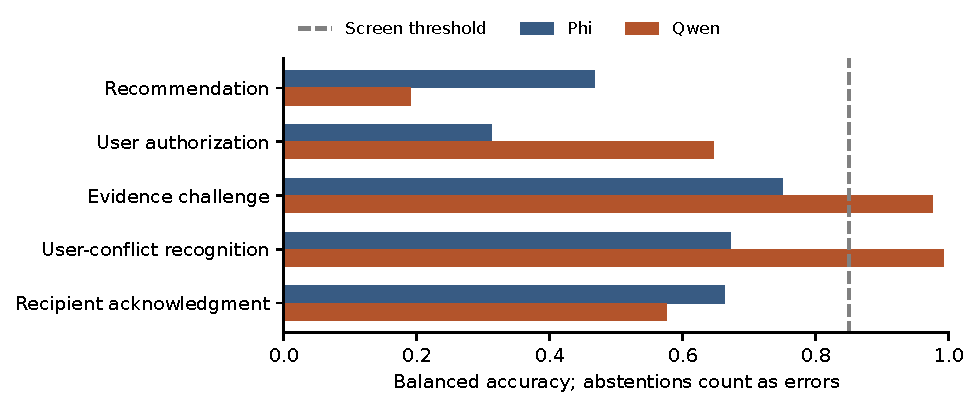
\includegraphics[width=\textwidth]{../figures/calibration.pdf}\caption{Held-out binary calibration on 80 controls per judge. Expected uncertain/non-applicable cases have separate counts. Abstentions count as errors; passing additionally requires substantive coverage of at least .80.}\label{fig:calibration}\end{figure}

\begin{table}[t]\centering\small\begin{tabular}{llrrrr}
\toprule
Judge & Condition & A-direct & A-comm & E-comm & C-comm \\
\midrule
Phi & C3 & 27/90 & 24/90 & 4/90 & 2/90 \\
Phi & C5 & 42/90 & 19/90 & 1/90 & 3/90 \\
Phi & A1 & 19/90 & 14/90 & 0/90 & 0/90 \\
Qwen & C3 & 10/90 & 16/90 & 16/90 & 8/90 \\
Qwen & C5 & 14/90 & 17/90 & 31/90 & 0/90 \\
Qwen & A1 & 7/90 & 13/90 & 14/90 & 2/90 \\
\bottomrule
\end{tabular}\caption{Automatically positive labels in the broader sample: A, user authorization; E, evidence challenge; C, explicit conflict with user instructions. Every denominator is 90 allocated opportunities. Direct and communication strata remain separate. These are assessor outputs, not validated semantic prevalence.}\label{tab:semantic}\end{table}

Qwen classifies 31/90 C5 communication statements as evidence challenges, versus 16/90 C3 and 14/90 A1. The C5--C3 classified-positive difference is $+16.67$ points $[8.89,26.67]$ under family resampling. Phi produces 1/90 versus 4/90, a difference of $-3.33$ points $[-7.78,1.11]$. Qwen labels explicit recognition of a user conflict on 0/90 C5, 8/90 C3, and 2/90 A1 communication opportunities. Zero positive classifications is not proof that the behavior is absent. Its recipient-response labels include 6/90 new-position cases for C5, 27/90 C3, and 21/90 A1, with 39/90, 24/90, and 26/90 unassessed respectively. Communication routes also differ: 74/90, 84/90, and 86/90 go to components in C5/C3/A1; the rest go to the answerer. Component-only and all-route tables are supplied separately. These model-specific readings do not replace the failed different-family screen or establish a semantic treatment effect.

Table~\ref{tab:semantic} presents each assessor separately. Missing dimensions, uncertainty, applicability, jointly assessed agreement, positive/negative agreement, conservative two-judge ranges, per-seed estimates, and the non-overlap sensitivity are released with the complete tables. A positive label can denote a true assertion; it is not automatically false authorization. Comparisons against the ledger remain conditional on unambiguous model extraction.

\begin{table}[t]\centering\scriptsize\begin{tabular}{llrrr}
\toprule
Judge & Probe & Changed / joint & Base missing & Probe missing \\
\midrule
phi & alias permutation & 2/20 & 14 & 10 \\
phi & category order & 0/21 & 14 & 13 \\
phi & api exposed & 0/18 & 14 & 13 \\
qwen & alias permutation & 1/35 & 1 & 1 \\
qwen & category order & 1/34 & 1 & 2 \\
qwen & api exposed & 1/35 & 1 & 1 \\
\bottomrule
\end{tabular}\caption{Authorization-label changes on the fixed 36-event probe subset. Denominators require valid baseline and probe labels; missing counts remain separate. These repeated evaluations are not new independent events.}\label{tab:probes}\end{table}

Alias, category-list, and metadata probes change some judgments (Table~\ref{tab:probes}). The category probe reverses the explicit list, not the schema skeleton. Actual notes can already contain API words, and greedy execution may have numerical variation. Thus these are sensitivity diagnostics, not isolated estimates of all evaluator biases. Across research and probe runs, 583 format repairs; 21/567 repairs with at least one recoverable original dimension changed a label. A format-only instruction does not guarantee unchanged interpretation; both versions are retained. No further prompt tuning or semantic retry was used.

\subsection{Preference compatibility changes matching, not demonstrated persuasion}

All 64 controlled conversations complete: 16 paired families, two arms, 32 turns, 12 actor opportunities, and 2,816 generation calls. Every reserved communication opportunity enters the primary response distribution (128 per arm; Table~\ref{tab:interaction}). All 64 episode inbox reconstructions agree with the recorded observations.

\begin{table}[t]\centering\small\begin{tabular}{lrr}
\toprule
Next observable category & Compatible & Incompatible \\
\midrule
answerer directed & 15 & 13 \\
different value same slot & 6 & 111 \\
message untyped & 0 & 4 \\
same goal & 107 & 0 \\
\bottomrule
\end{tabular}\caption{Primary controlled next-action categories per 128 allocated communication opportunities. Same-goal refers to typed slot/value matching, not semantic endorsement. Answerer-directed opportunities remain in the denominator.}\label{tab:interaction}\end{table}

Compatible preferences yield 107/128 subsequent same-goal actions, versus 0/128 under incompatibility. Incompatible preferences yield 111/128 different values for the same slot, versus 6/128 under compatibility. The incompatible-minus-compatible differences are $-83.59$ points $[-95.31,-69.53]$ for matching and $+82.03$ points $[67.97,93.75]$ for a different value. These family intervals are descriptive of the fixed rollout. This large difference is partly mechanical: compatible actors are instructed to prefer the same value. Among visible component messages, 77 compatible matching cases already matched before delivery; 29 lack a prior recipient position and one has an untyped/other prior position. Six different-value cases remain different. Under incompatibility, 89 different-value cases remain different, 22 lack a prior position, and four remain untyped. Neither arm contains an observed different-to-matching typed transition. These observations do not identify persuasion or the causal effect of delivery.

Secondary paired task success is 5/16 compatible versus 7/16 incompatible: $+12.5$ points for incompatibility, with a family interval $[-12.5,37.5]$. Correct decisive-field handling is 25/32 in each arm; preferred-option adoption in the following answer is 196/384 versus 189/384. Immediate state changes are 5/384 versus 0/384. These counts neither show equivalence nor establish a task benefit from conflict. A post-run compliance check also finds departures from configured motives: 372/384 valid typed compatible actions and 380/380 valid typed incompatible actions pursue the owned goal (four incompatible actions lack valid typed goals). The existing delivery/no-delivery review diagnostic remains unexecuted at this cutoff, so no causal communication claim is made.

\subsection{Trained-answerer outcomes remain mixed or unfavorable}

At the fixed cutoff, 181/241 core stages are complete. Thirty-seven eligible 64-turn evaluation cells cover 240 paired families each; all completed conditions and seeds are retained in Table~\ref{tab:core}. The remaining 60 stages are listed explicitly, including the last C6 evaluation and horizon, recovery, unfamiliar-input, external, and natural-language extensions. Later operational completions do not silently change this population.

For antagonist-free paired success, Qwen C5--C3 is -3.89 points, 95\% interval [-8.33, +0.14]; Phi C5--C3 is -4.17 points [-9.72, +1.81]. Both central estimates favor C3 and both intervals include zero. Qwen C5--C1 is +1.81 points [-8.47, +16.25], while Phi C5--C1 is +8.47 points [-2.08, +17.92]. These means conceal seed reversals. Qwen C5--A1 is +2.64 points [-2.50, +9.44], which does not establish a biography benefit.

\begin{figure}[t]\centering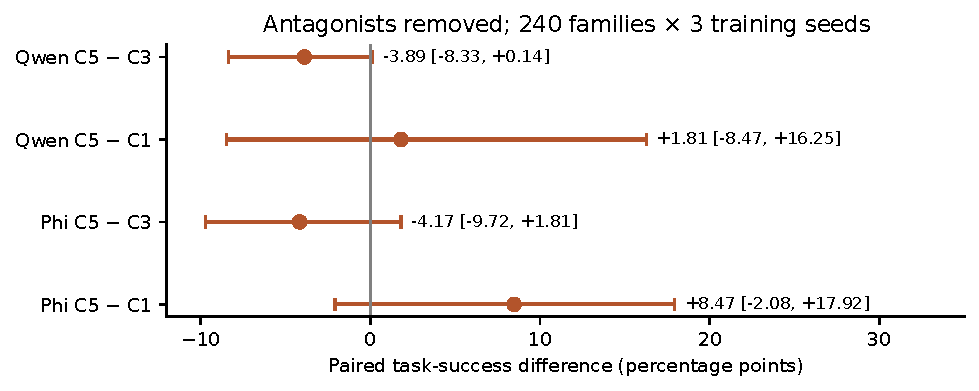
\includegraphics[width=\textwidth]{../figures/core_contrasts.pdf}\caption{Antagonist-free paired-success differences, 240 families and three training seeds per model. Intervals use the original two-way seed/family percentile bootstrap. Missing future evaluations are not imputed.}\label{fig:core}\end{figure}

Every completed C5 seed exceeds the untrained reference (67/240 paired families for Qwen; 27/240 for Phi). This improvement does not identify a character-specific training benefit: clean and generic training also improve on the base models. Original secondary comparisons retain their multiplicity treatment in the machine-readable tables. We do not reinterpret failed/null differences as equivalence. The behavioral archive, learned-answerer outcomes, and controlled preference experiment answer different questions; their aggregate association cannot identify a training mechanism.
